\documentclass{article}
\usepackage[utf8]{inputenc}
\usepackage[portuges]{babel}
\usepackage{csquotes}
\usepackage{geometry}
\usepackage[pdftex]{hyperref}
\usepackage{indentfirst}
\usepackage{amsthm}
\usepackage{amssymb}
\usepackage{amsmath}
\usepackage{mathrsfs}
\usepackage{graphicx}
\usepackage{float}
\usepackage{multicol}
\usepackage{verbatim}
\usepackage{dsfont}

\newtheorem{definition}{Definição}
\newtheorem{theorem}{Teorema}
\newtheorem{lemma}[theorem]{Lema}
\newtheorem{example}{Exemplo}

\usepackage[backend = biber]{biblatex}
\addbibresource{quarto_trabalho.bib}

\geometry{left = 3cm, top = 3cm, bottom = 2cm, right = 2cm}

\title{Inferência Estatística \\ 4º Trabalho}
\author{Igor Patrício Michels}
\date{18/11/2020}

\begin{document}

\maketitle

\section*{Introdução}

Trabalho elaborado pelo aluno Igor Patrício Michels referente a disciplina de Inferência Estatística, do quarto período da Graduação em Matemática Aplicada da FGV-EMAp. Nele iremos abordar o conceito de teste uniformemente mais poderoso.

O enunciado e eventuais funções utilizadas para resolução deste ou de outros trabalhos podem ser encontrados \href{https://github.com/IgorMichels/Statistical_Inference}{\textbf{nesse repositório do GitHub}}.

\section*{Teste Uniformemente Mais Poderoso}

\subsection*{Contextualizando}\label{contexto}

Em 2008 fui passar minhas férias em Gotham City. Confesso que as férias não foram das melhores, a cidade estava um caos. Aparentemente um palhaço não gostava de morcegos e estava numa tremenda batalha com um tal de homem morcego. Pelo que soube esse tal homem morcego era uma espécia de herói na cidade. Certo dia eu estava caminhando pela rua e encontrei um possível vítima desse palhaço, ele havia explodido um hospital no dia anterior. O homem que encontrei parecia ter saído de um transplante facial, o qual não tinha sido finalizado e o homem estava meio cara, meio... coroa. Acho que ele ão foi com minha cara quando perguntei por que ele estava dessa forma e disse que iria lançar sua moeda e, se o resultado fosse $C$ (cara), me daria uns cascudos. Tentei chamar esse tal de homem morcego, mas parece que aquele palhaço estava interessado em explodir uns barcos, então quem sou eu no meio dessa crise toda? Achei válido o tal do homem morcego se interessar em evitar as explosões. No fim, acabei pedindo para esse cara da moedinha decidir se me daria os cascudos pela moeda mesmo mas antes lançar a moedas algumas vezes para mim ter uma ideia do meu futuro. Surpreendentemente ele aceita, falando que sou um cara engraçado então poderia me fazer esse favor, mas que eu não escaparia dessa sem ele lançar a moeda. Ele lançou a moeda $10$ vezes e obteve a sequência
\[\text{KCKCKCCKKK}.\]

Como ele caiu na minha e fez esses lançamentos pude fazer alguns testes a respeito da moeda e analisar se valeria a pena tentar fugir desse sujeito, talvez tomando dois cascudos por isso, ou se ficaria e deixaria o destino a cargo da moeda.

Antes de ver o que aconteceu comigo, vamos ver algumas definições e ideias.

\subsection*{Teste UMP e MLR}

Conforme subseção anterior, iremos, nessa subseção,  tomar algumas definições e ideias, as quais também podem ser encontradas no DeGroot \cite{degroot}.

Sejam $\delta$ um procedimento de teste, $\alpha(\delta)$ o tamanho do teste $\delta$ e $\pi(\theta \mid \delta)$ a função poder do teste, podemos definir um Teste Uniformemente Mais Poderoso como
\begin{definition}[Teste Uniformemente Mais Poderoso]
    Dadas duas hipóteses $H_0 : \theta \in \Omega_0$ e $H_1 : \theta \in \Omega_1$ dizemos que um procedimento $\delta^*$ é uniformemente mais poderoso sob as hipóteses $H_0$ e $H_1$ no nível de significância $\alpha_0$ se $\alpha(\delta^*) \leq \alpha_0$ e, para todo procedimento $\delta$ de modo que $\alpha(\delta) \leq \alpha_0$, vale que
    \[\pi(\theta \mid \delta) \leq \pi(\theta \mid \delta^*), \forall ~\theta \in \Omega_1.\]
\end{definition}

Uma outra definição importante se é a definição de Razão de Verossimilhança Monotônica
\begin{definition}[Razão de Verossimilhança Monotônica]
    Seja $f_n(x \mid \theta)$ a função de densidade conjunta das observações $X = \left(X_1, ~X_2, ~\dots, ~X_n\right)$ e $T = r(X)$ uma estatística. Dizemos que a distribuição conjunta de $X$ tem razão de verossimilhança monotônica (MLR) na estatística $T$ se para todo par de valores $\theta_1, \theta_2 \in \Omega$, com $\theta_1 < \theta_2$, a razão
    \begin{equation}
        \label{MLR}
        \dfrac{f_n(x \mid \theta_2)}{f_n(x \mid \theta_1)}
    \end{equation}
    
    \noindent depende do vetor de observações apenas por meio da estatística $T$ e a razão acima é uma função monótona de $T$ na imagem de $r(x)$.
\end{definition}

Por fim, podemos fazer uma última definição
\begin{definition}[Razão de Verossimilhança Monotônica Crescente e Razão de Verossimilhança Monotônica Decrescente]
    Dizemos que $X$ tem Razão de Verossimilhança Monotônica Crescente quando a razão \ref{MLR} é crescente e que $X$ tem Razão de Verossimilhança Monotônica Decrescente quando a razão \ref{MLR} é decrescente.
\end{definition}

Dadas tais definições, podemos enunciar alguns Teoremas.
\begin{theorem} \label{teo1}
    Tome $\delta^*$ um procedimento em que a hipótese $H_0$ não é rejeitada se $a f_0(x) > b f_1(x)$ e a hipótese $H_0$ é rejeitada se $a f_0(x) < b f_1(x)$. Para o caso em que $a f_0(x) = b f_1(x)$ a hipótese $H_0$ pode ser tanto rejeitada quanto não rejeitada. Então, para todo outro procedimento de teste $\delta$ vale que
    \[a \alpha(\delta^*) + b \beta(\delta^*) \leq a \alpha(\delta) + b \beta(\delta).\]
\end{theorem}

\begin{proof}
    A cargo do leitor.
    \vspace{12pt}
    
    \noindent Dica: Veja a seção 9.2 do DeGroot \cite{degroot}.
\end{proof}

Visto esse teorema, temos o ferramental para provar um outro Teorema:

\begin{theorem}[Lema de Nayman-Pearson]\label{teo2}
    Suponha que $\delta^*$ é um procedimento de teste que, dada uma constante $k > 0$, a hipótese $H_0$ não é rejeitada se $f_1(x) < k f_0(x)$ e é rejeitada se $f_1(x) > k f_0(x)$. Caso $f_1(x) = k f_0(x)$ a hipótese $H_0$ pode tanto ser rejeitada quanto não rejeitada. Se $\delta$ é um outro procedimento de forma que $\alpha(\delta) \leq \alpha(\delta^*)$, então $\beta(\delta) \geq \beta(\delta^*)$. Além disso, se $\alpha(\delta) < \alpha(\delta^*)$, então $\beta(\delta) > \beta(\delta^*)$.
\end{theorem}

\begin{proof}
    Pelo Teorema \ref{teo1}, temos que
    \[k \alpha(\delta^*) + \beta(\delta^*) \leq k \alpha(\delta) + \beta(\delta) \implies k \left(\alpha(\delta^*) - \alpha(\delta)\right) + \beta(\delta^*) \leq \beta(\delta).\]
    
    \noindent Agora, como $\alpha(\delta) \leq \alpha(\delta^*)$, vale que $k \left(\alpha(\delta^*) - \alpha(\delta)\right) \geq 0$, logo, temos que $\beta(\delta) \geq \beta(\delta^*)$. Em especial, se $\alpha(\delta) < \alpha(\delta^*)$, vale que $k \left(\alpha(\delta^*) - \alpha(\delta)\right) > 0$ e então decorre que $\beta(\delta) > \beta(\delta^*)$.
\end{proof}

\begin{theorem}\label{teo3}
    Seja $H_0 : \theta = \theta_0, ~\theta_0 \in \Omega$ uma hipótese simples. Se vale o Teorema da Fatoração e existem $c$ e $\alpha_0$ de modo que
    \[P(r(X) \leq c \mid \theta = \theta_0) = \alpha_0,\]
    
    \noindent então o procedimento $\delta^*$ que rejeita $H_0$ se $r(X) \leq c$ é UMP para $H_0$ ao nível $\alpha_0$.
\end{theorem}

\begin{proof}
    Em primeiro lugar, considere o procedimento $\delta'$, teste de razão de verossimilhança de nível $k \in (0, 1)$, isto é, o teste em que rejeitamos $H_0$ se $\Lambda(x) \leq k$. Dessa forma
    \begin{equation*}
        \begin{split}
            \Lambda(x) \leq k & \iff \dfrac{\sup_{\theta_0 \in \Omega_0} f_n(x \mid \theta)}{\sup_{\theta \in \Omega} f_n(x \mid \theta)} \leq k \\
            & \overset{(1)}{\iff} \dfrac{f_n\left(x \mid \theta_0\right)}{f_n\left(x \mid \hat{\theta}\right)} \leq k \\
            & \overset{(2)}{\iff} \dfrac{u(x)\cdot v\left(r(x), \theta_0\right)}{u(x)\cdot v\left(r(x), \hat{\theta}\right)} \leq k \\
            & \iff \dfrac{v\left(r(x), \theta_0\right)}{v\left(r(x), \hat{\theta}\right)} \leq k \\
            & \iff v\left(r(x), \theta_0\right) \leq k\cdot v\left(r(x), \hat{\theta}\right).
        \end{split}
    \end{equation*}
    
    Agora, fazendo $v\left(r(x), \theta_0\right) = f_1(x)$ e $v\left(r(x), \hat{\theta}\right) = f_0(x)$, dessa forma, podemos dizer que o teste que estamos realizando é equivalente ao teste que não rejeita $H_0' = H_1$ se $f_1(x) \leq k\cdot f_0(x)$. Mas, pelo Teorema \ref{teo2}, isso implica que para todo outro procedimento de teste $\delta$, vale que 
    \[\beta(\delta) \geq \beta(\delta'),\]
    
    \noindent o que nos mostra que o procedimento $\delta'$ é um teste UMP.
    
    Agora iremos mostrar que $\delta'$ equivale a $\delta^*$.
    
    Caso $\theta_0 = \hat{\theta}$, teremos que a razão de verossimilhança será igual a $1$ e, com isso, não rejeitamos a hipótese nula. Agora, caso contrário, podemos escrever $\theta_0 = g_1(r(X))$ e $\hat{\theta} = g_2(r(X))$, além de supor que $\theta \in \mathds{R}$. Se $\theta_0 < \hat{\theta}$, temos que a razão de verossimilhança será monotônica. Dessa forma, reescrevemos
    \[\dfrac{v\left(r(x), g_1(r(X))\right)}{v\left(r(x), g_2(r(X))\right)} \leq k,\]
    
    \noindent de onde vemos que a razão depende apenas da imagem de $r(X)$, então podemos tirar uma relação do tipo $r(x) \leq c$. Caso contrário, isto é, $\theta_0 > \hat{\theta}$, a razão
    \[\dfrac{v\left(r(x), g_2(r(X))\right)}{v\left(r(x), g_1(r(X))\right)} \geq \dfrac{1}{k},\]
    
    \noindent também é monotônica dependendo apenas da imagem de $r(X)$, valendo o mesmo que o caso anterior. Dessa forma, conclui-se que os testes $\delta^*$ é equivalente a $\delta'$, ou seja, $\delta^*$ como descrito no enunciado é UMP.
\end{proof}

\subsection*{Voltando a nosso contexto}

Uma vez que aquele sujeito aceitou lançar a moeda $10$ vezes pude realizar um teste de hipóteses. Como eu levaria um cascudo caso o resultado fosse C, é interessante analisar as hipóteses $H_0 : p \leq \frac{1}{2}$ e $H_1 : p > \frac{1}{2}$, onde $p$ é a probabilidade de eu me dar mal.\footnote{Ou seja, dar cara e eu levar uns cascudos.}

Note que esse caso se dá por $10$ lançamentos independentes de uma moeda com probabilidade $p$ de resultar cara, dessa forma, o espaço de parâmetros se dá pelo intervalo $\Omega = [0, 1]$ e, além disso, temos $\Omega_0 = \left[0, \frac{1}{2}\right]$. Dessa forma, podemos escrever a razão de verossimilhança como
\[\Lambda(x) = \dfrac{\sup_{\theta_0 \in \Omega_0} f_n(x \mid \theta)}{\sup_{\theta \in \Omega} f_n(x \mid \theta)}.\]

Mas aqui estamos tratando de variáveis Bernoulli, onde sabemos que a quantidade de caras resultantes é uma estatística suficiente, então podemos reescrever
\begin{equation*}
    \begin{split}
        \Lambda(x) & = \dfrac{\sup_{\theta \in \Omega_0} \binom{n}{y} \theta^y(1 - \theta)^{n - y}}{\sup_{\theta \in \Omega} \binom{n}{y} \theta^y(1 - \theta)^{n - y}} \\
        & = \dfrac{\sup_{\theta \in \Omega_0} \theta^4(1 - \theta)^6}{\sup_{\theta \in \Omega} \theta^4(1 - \theta)^6},
    \end{split}
\end{equation*}

\noindent onde é fácil ver que $\theta_0 = \theta = \frac{2}{5}$, dessa forma
\[\Lambda(x) = \dfrac{\left(\frac{2}{5}\right)^4\left(1 - \frac{2}{5}\right)^6}{\left(\frac{2}{5}\right)^4\left(1 - \frac{2}{5}\right)^6} = 1,\]

\noindent onde vemos que a hipótese $H_0$ não seria rejeitada no teste de razão de verossimilhança.

Além disso, reescrevendo essa razão de verossimilhança como 
\[\Lambda(x) = \dfrac{\theta_0^y(1 - \theta_0)^{n - y}}{\hat{\theta}^y(1 - \hat{\theta})^{n - y}} = \left(\dfrac{\theta_0\left(1 - \hat{\theta}\right)}{\hat{\theta}\left(1 - \theta_0\right)}\right)^y \left(\dfrac{1 - \theta_0}{1 - \hat{\theta}}\right)^n,\]

\noindent onde podemos ver que temos uma razão de verossimilhança monotônica na estatística $y$, que representa a quantidade de caras que foram obtidas. Dessa forma, aplicando, de forma adaptada para o caso discreto, o teorema 9.3.1 do DeGroot \cite{degroot}, temos que o teste que rejeita $H_0$ no nível $\alpha_0$ é o teste que rejeita $H_0$ se $y \geq c$, onde $c$ é tal que
\[P\left(y \leq c \mid \theta = \dfrac{1}{2}\right) = \alpha_0.\]

Tomando $\alpha_0 = 0.1$, temos que iremos rejeitar $H_0$ se $y \geq 8$, sendo esse um teste UMP para esse caso. Como obtivemos um total de $4$ caras, não temos como rejeitar a hipótese $H_0$, dessa forma, optei não fugir do sujeito que queria me dar uns cascudos.

Entretanto, apesar do teste não rejeitar a hipótese de que $\theta_0 \leq \frac{1}{2}$, surgiu uma outra oportunidade para mim\footnote{Curiosamente, uma outra jogada de sorte!}, um outro homem estava se aproximando de nós dois com uma sacola de moedas a serem trocadas, então pensei ``esse sujeito aí só pode decidir se vai me dar uns cascudos através da moedinha se ele souber qual a moedinha'', dessa forma, quando o homem que estava com a sacola de moedas se aproximou eu pedi para que ele decidisse sobre meu cascudo e, enquanto a moeda estava no ar, lancei a sacola de moedas no ar e saí correndo enquanto o sujeito lá buscava por sua moedinha.

Moral: o teste de hipóteses me inclinou a aceitar que ele lançasse a moedinha para ver minha sorte, mas minha sorte foi, na verdade, o homem com a sacola de moedas!

\subsection*{Desafio ao leitor}

Facilmente podemos ver que no nosso contexto não podemos atingir qualquer nível $\alpha_0$. Isso se dá pelo fato de estarmos trabalhando com variáveis discretas, ou seja, nossa função é uma função ``escada'', cheia de degraus, veja a Figura \ref{binomial} para uma ilustração desse fato.
\begin{figure}
    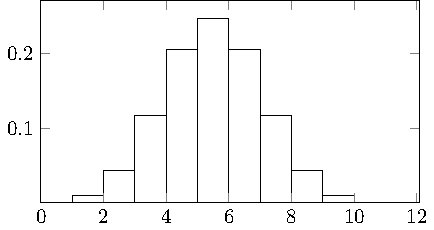
\includegraphics[page = 1]{Tikz.pdf}
    \includegraphics[page = 2]{Tikz.pdf}
    \caption{à esquerda, com a ideia de ilustrar, temos a plotagem da densidade de uma $\operatorname{Bin}(10, 0.5)$ em forma de histograma, já à direita a plotagem da acumulada da mesma.}
    \label{binomial}
\end{figure}

Note que nem toda reta do tipo $y = \alpha_0$ intersecta a função de probabilidade acumulada, ou seja, nem sempre podemos encontrar um valor $k$ de forma que a acumulada da distribuição tenha imagem $\alpha_0$. Como exemplo, se traçarmos a reta $y = 0.1$, como se estivéssemos considerando $\alpha_0 = 0.1$, não temos nenhum ponto $k$ que nos dê um teste de nível $0.1$ no experimento descrito anteriormente.

A ideia aqui é que você proponha uma solução para isso, ou seja, mostre como podemos fazer nosso teste de modo que possamos atingir qualquer nível $\alpha_0$ em $(0, 1)$.

\section*{Conclusão}

Em primeiro lugar, pude concluir nas férias que palhaços e bananas pode resultar numa combinação explosiva. Além disso, vi que a frase ``nunca fale com estranhos na rua'' realmente é muito válida e que moedas, além de facilitarem seu troco, podem te auxiliar a sair de algumas furadas, embora possam te colocar em outras.

Fora essas conclusões, podemos ver que, em alguns casos, é mais simples e eficaz realizar um procedimento de teste a partir de uma estatística suficiente, tanto pela simplicidade do teste quanto pelos resultados, principalmente quando esse procedimento for UMP. Note que basta comparar a estatística com um valor real para rejeitar ou não a hipótese nula, ou seja, é um teste relativamente simples de ser aplicado.

Já pelos resultados, vimos que um teste UMP busca minimizar as probabilidades de erros, dessa forma aplicar um teste UMP, quando possível, pode ser muito relevante para a análise que desejamos fazer, principalmente quando um erro pode ser crucial como, por exemplo, nos testes de eficiência para uma nova droga.

\section*{Resposta do desafio}

Essencialmente, a solução do desafio proposto é aplicar uma ideia probabilística ao teste. Ou seja, dado um nível $\alpha_0$ se encontrarmos $c$ de forma que
\[P(r(X) \geq c \mid \theta = \theta_0) = \alpha_0,\]

\noindent está perfeito e temos nosso teste pronto. Caso contrário, isto é, se não existe $c$ que satisfaça a relação acima, podemos encontrar um valor $c$ tal que
\[P(r(X) \geq c \mid \theta = \theta_0) < \alpha_0 \text{ e } P(r(X) \geq c + 1 \mid \theta = \theta_0) > \alpha_0.\]

Agora, nesse momento, rejeitando $H_0$ caso $r(X) \geq c$, o tamanho do teste será menor que $\alpha_0$, mas rejeitando $H_0$ quando $r(X) \geq c + 1$, o tamanho será maior que $\alpha_0$. Então uma solução para termos um teste de tamanho $\alpha_0$ é rejeitar $H_0$ se $r(X) \geq c$ e, se $r(X) = c + 1$, rejeitar $H_0$ com uma probabilidade $q$, a qual será escolhida de forma que
\[q\cdot P(r(X) = c + 1 \mid \theta = \theta_0) + P(r(X) \geq c \mid \theta = \theta_0) = \alpha_0.\]

Uma ilustração disso é como se, quando $r(X) = c$, a gente lançasse uma ``moeda''\footnote{Moedas aparecendo de novo...} com probabilidade $q$ de sair cara. Tendo o resultado dessa moeda, rejeitamos $H_0$ se o resultado for cara e não rejeitamos se for coroa.

\printbibliography

\end{document}